%\documentclass[a4paper]{IEEEtran}
\documentclass[a4paper, onecolumn, 11pt]{article}
\usepackage[T1]{fontenc}
\usepackage[utf8]{inputenc}
\usepackage[english]{babel}

\usepackage{authblk}
\usepackage{hyperref}
\usepackage{graphicx}
\usepackage{listings}
%\usepackage{amsmath}
\usepackage[cmex10]{amsmath}
\usepackage{amssymb}
\usepackage{fullpage}
\usepackage{float}
\usepackage{url} \urlstyle{sf}

\usepackage{dashrule}

\usepackage{color}
\usepackage{caption}
\usepackage{subcaption}
\newcommand{\alert}[1]{\color{red}{#1}}
\newcommand{\greyout}[1]{\color{gray}{#1}}

\setlength{\parskip}{0.75em}

\title{Specifying the Experimental Scenarios for Simulated Cloud Studies}
%TODO 2 part in experiment, the static 
%\author{
%	\IEEEauthorblockN{Simon Bihel (Student)\IEEEauthorrefmark{1} \footnote{Work 
%	done during this author's internship.} \and
%    Martin Quinson\IEEEauthorrefmark{1}\IEEEauthorrefmark{3} \and
%    Anne-C\'ecile Orgerie\IEEEauthorrefmark{2}\IEEEauthorrefmark{3}}\\
%	\IEEEauthorblockA{
%    \hspace{1cm}\IEEEauthorrefmark{1}Dept. of Computer Science, ENS Rennes\\
%  	\hspace{1cm}\{firstname.lastname\}@ens-rennes.fr}\\
%  \IEEEauthorblockA{
%    \IEEEauthorrefmark{2}CNRS\\
%    anne-cecile.orgerie@inria.fr}\\
%  \IEEEauthorblockA{
%    \IEEEauthorrefmark{3}Myriads team, IRISA}
%}
\author{Simon Bihel \\ Dept. of Computer Science, ENS Rennes\\
  \href{mailto:simon.bihel@ens-rennes.fr}{simon.bihel@ens-rennes.fr}}


\begin{document}
\maketitle

\begin{abstract}
  Cloud computing is a model that makes available infrastructures, platforms and
  software with a pay-as-you-go subscription. It aims to reduce the cost with a
  layer of visualization that allows virtual resources to be dynamically
  adjusted and occupied on-demand. The problem of using the minimal resources
  for the current demand/usage is still a research challenge that spans all
  layers and applications. This dynamic management of clouds is called cloud
  elasticity. To evaluate research work done on cloud elasticity simulation can 
  be used and presents some advantages. While the simulation of cloud 
  structures are already possible there is a lack of workload generation which 
  is essential to evaluate works supposed to deal with fluctuating workload. 
  This paper presents a way of describing workloads using tasks that are 
  repeated over time with parameters that can be modified over time. It also 
  shows that this proposition fits the needs of past works.
\end{abstract}

%\begin{IEEEkeywords}
%  Simulation;
%  Workload;
%  Cloud elasticity
%\end{IEEEkeywords}
\providecommand{\keywords}[1]{\textbf{\textit{Index terms---}} #1}
\keywords{Simulation; Workload; Cloud elasticity}

\section{Introduction} \label{intro}
  Nowadays clouds are used for a lot of server-based applications. From websites
  to scientific computing, it allows apps creators to avoid managing their own
  servers. Because of a well defined business model the cloud structure is
  composed of layers where each layer uses the precedent one and provides a
  service to the next one. The services provided by a layer is negotiated (e.g.
  to determine the pricing) and levels of quality have to be met. Of course the
  goal is to meet these levels of quality while minimizing the costs like the
  usage of the bottom layer, energy consumption... Research is being done to
  tackle this problem. The domain we are particularly interested in is the one
  that deals with fluctuating usage where dynamic management is required to
  minimize costs at all time.
  
  As clouds are complex structures these works have to be evaluated. Theory is
  not enough as so many problems are NP complete. One way is to use a real cloud
  and deploy the work that should be tested, and then generate somewhat
  artificial workload for the app. Another way of doing it would be to simulate
  the cloud and the workload. This kind of evaluation has often been used for
  grids, which can be seen as the ancestor of clouds. Among the different
  advantages of simulations, simplicity would come up on top.
  
  For now it is possible to simulate clouds infrastructures but tasks are still
  seen as individual and independent computing task. For elastic clouds research
  it is essential to generate authentic workload and there is currently no way
  of manipulating naturally workloads for simulations. During this internship we
  worked on writing an API for SimGrid and this paper presents the work done.
  
  In \ref{background} we give a more detailed presentation of clouds and their 
  uses. In \ref{sota} we study the work done on simulation, workload generation 
  and define in more details the needs for a workload generator based on past 
  work on cloud elasticity. \ref{contrib} presents the actual contribution and 
  its use. \ref{eval} provides an evaluation based on performances and 
  expressiveness to make sure the contribution fits the needs. \ref{conclu} 
  concludes on whether this contribution will help future research.
  
  The main contributions of this internship are: (i) a categorization and
  generalization of experimental needs for this domain; (ii) an implementation
  of an API to evaluate this categorization.


\section{Background} \label{background}
	%TODO add subsections, cloud computing, typical cloud studies, experimental 
	%methodologies
  \begin{figure*}
    \caption{Cloud architecture. \\ 
    \url{http://cloud-simulation-frameworks.wikispaces.asu.edu/}}
    \centering
    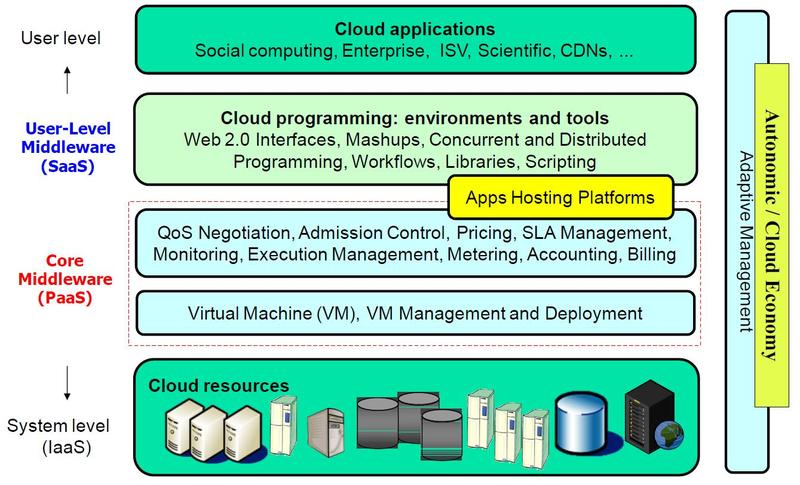
\includegraphics[width=0.7\textwidth]{../plots/cloud_architecture}
    \label{cloud_arch}
  \end{figure*}
  
  \figurename~\ref{cloud_arch} describes the global architecture of a cloud. It
  is split in different layers and each layer has a specific role in the model
  of clouds. On the lowest part there is the physical resources (e.g. data
  centers) with Infrastructure as a Service model (IaaS). The pricing is based
  of the resources available. Then comes the layer of virtualization and
  performances negotiation called Platform as a Service (PaaS). Dealing with
  Virtual Machines (VMs also called hosts) allows a cleaner sharing of resources
  and makes it easier answering the users' demands (e.g. deploying more VMs).
  The pricing depends of multiple factors, like the Quality of Service (QoS) for
  the quality of the network, the Service Level Agreement (SLA) for the faults
  rate, handling and responsibilities... On top of that is the layer for users'
  cloud tools with Software as a Service (SaaS). These tools will allow the user
  that writes cloud applications to manage resources, run their code... This 
  architecture and organization is a real enhancement as before that users 
  would have to run their own application stack (e.g. managing servers, 
  databases, etc.). In addition to that the pay-as-you-go business models makes 
  it even more convenient for the user to react, increase capacities, try new 
  features, get more control on certain layers (e.g. for optimization purpose), 
  etc.
  
  Cloud applications will have fluctuating workload over time. For example with
  a website server the usage will be bigger during the day or during a short
  period because of a viral cultural event. Resources should thus be managed
  dynamically. Also, physical resources can encounter problems which makes them
  unavailable. Because of all these constraints the SLAs and QoS negotiations
  are not satisfied easily and 100\% availability is never a thing. On top of
  that every actor wants to meet the obligations with a minimal cost. All these
  questions of availability and cost are current research problems. In
  particular we are interested in the works that tackle problems related to
  fluctuating and dynamic usage of cloud applications and resources. The ability
  for a cloud infrastructure to adapt to a dynamic workload is called cloud
  elasticity.
  
  %TODO paragraph about the major problem is optimization (response time, cost)
  
  There are some generic elastic actions. The act of deploying more VMs (and
  thus having more resources overall) is called scaling up (and the convert is
  scaling down). The act of moving VMs to a different location is called scaling
  out. This is used for example when time passes by and users come from
  different countries/continents.
  
  %TODO say that there are multiple things to evaluate (theory, simulation e.g.)
  
  \cite{Naskos2016} has categorized works on cloud elasticity and allows to see
  which elements of a cloud infrastructure (platform or application/software)
  are impacted. As it is for now most research works are evaluated on real
  clouds. It is interesting for a distributed systems simulator to search what
  is needed for simulating cloud elasticity. If it is shown that research works
  on cloud elasticity can be evaluated on a simulator they would benefit from
  simple setups, cost reduction, reproducible experiments, trust in results... 
  These are particularly important when comparing two algorithms, which is a
  good part of this domain. Again, theory is not enough to study a cloud
  software (e.g. a scheduler) as there are too many NP complete problems.
  
  In this survey proposals are categorized as follows. The scope is about what
  elements of a cloud the proposals work on. It can be the management of VMs,
  allocation of resources... Then there is the purpose of the proposal.
  Enhancing the \textit{performances} (to meet the SLA), reducing the
  \textit{energy consumption} footprint, being \textit{available} when needed
  and reducing the overall \textit{cost}. Another dimension is the decision
  making. This is what a proposal add to an existing cloud to reach its goal. In
  addition to the scope there is the elastic actions performed by the proposals.
  As the scope is about what elements of a cloud are concerned, the elastic
  action is about what is done to them. Then there is the provider dimension
  that tells if there is only one provider or multiple ones. At last there is
  the method used by the proposal to evaluate itself, through real cloud,
  simulation or emulation.
  
  The survey gives a good overview on what elements of a cloud are manipulated
  to achieve cloud elasticity. No clue have been found proving the opposite at
  the time of writing.
  
  About simulators and particularly SimGrid. At first they are discrete event 
  simulators. They have a queue of events and jump between following events 
  thus not doing anything when the state of simulation remains constant. For 
  cloud or grid simulator one of these events will be tasks (AKA jobs, 
  gridlets, cloudlets, etc.) that will require a certain amount of flops (or 
  another resource unit) to be completed. As they don't really execute these 
  computing tasks, the completion of a task will be an event and if there is 
  another task queued up it will start. If the simulated platform can handle 
  easily the tasks then the simulator will have no problem to simulate this 
  smooth execution. But if too much tasks are queued up the simulator will use 
  a lot of memory to keep track of every element's state.
    
  As the proposals are on reacting to variating usage, simulators need a way to
  express this fluctuating workload. We worked on elastic tasks that model tasks
  that are triggered regularly and with a usage that fluctuates over time.


\section{Contribution} \label{contrib}
  %TODO seperate the scientific needs and the technical
  The work was done on SimGrid \cite{casanova:hal-01017319}. The code is
  available here: \url{https://github.com/sbihel/internship_simgrid}. It was
  written as a plug-in on top of the S4U interface which is intended to be the
  core API. Elastic tasks (ETs) are objects and are the only things the user has
  to manipulate.
  
  %TODO we see workload as a discrete stuff
  One key notion is that we use a discrete representation of workloads. Even if 
  workloads are generated by a discrete amount it is easier for cloud 
  elasticity researchers to see the workload as a continuous function of flops. 
  If we still decided to ..... because discrete event simulator
   
  An elastic task can repeat a certain task that we will call microtask. The 
  user provides a rate of triggering per second and the flops required and then 
  over time multiple identical microtasks will be created and executed. An 
  elastic task can have multiple hosts to split the workload and there will be 
  a cycling shifting between hosts when creating microtasks, keeping one host 
  for one microtask.
  
  An output function can be provided to an elastic task and this function will 
  be executed after each microtask that has ended. This has multiple usages. It 
  allows the description of workflows of tasks. As microtasks only generate 
  computing workload, output functions can be used to have different types of 
  workloads like network usage, disk access (which can be simulated only by 
  seeing it as a particular computing resource at the moment), and basically 
  anything possible with SimGrid.
  
  It is also useful to study the behavior of a system dealing with real 
  workload. For that an elastic task can be given a file of timestamps and it 
  will trigger/generate a microtask for each time stamp.
  
  For detailed platforms description it is a core feature of SimGrid which 
  allows to have multiple providers, topologies, hosts (VMs for us), 
  bandwidths... % say that this is not specific to cloud


\section{Evaluation} \label{eval}
  The contribution has been evaluated on the predefined criteria. We first did 
  an experiment for raw performances. Then we used real traces from WorldCup 98 
  data access logs \cite{wc98} which are often used. After that we evaluated 
  the expressiveness and functionalities. All experiments have been executed on 
  a MacBook Pro with an Intel Core i5 and 8GB of RAM.
    
  \subsection{Raw performances} \label{raw_perf}
    We evaluate raw performances to make sure that users can do significant 
    experiments. Basically we just want to see if the time and memory used grow 
    linearly with the number of micro tasks so that it can be used on a regular 
    computer and allows multiple quick experiments.
  
  	Two different experiments were made. During first one the number of elastic 
  	tasks grows while keeping a ratio of one ET per host and one trigger per 
  	second. The sole purpose of this is to see the performances because a 
  	typical cloud app will use about 15 ETs. For the second experiment it's the 
  	number of triggering per second that grows while keeping only one ET with 
  	200 hosts.
    
    \paragraph{Experiment 1}
    \begin{figure}
    	\centering
    	\hspace*{-4em}
    	\begin{subfigure}[t]{0.6\textwidth}
    		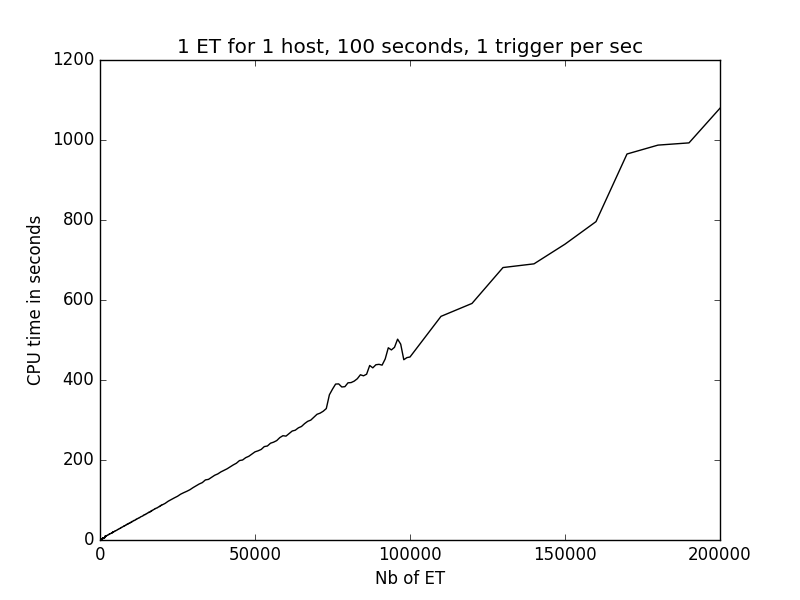
\includegraphics[width=\textwidth]{../plots/raw_perf_time}
    		\caption{Raw performances CPU time.}
    		\label{time_raw}
    	\end{subfigure}%
    	~
    	\begin{subfigure}[t]{0.6\textwidth}
    		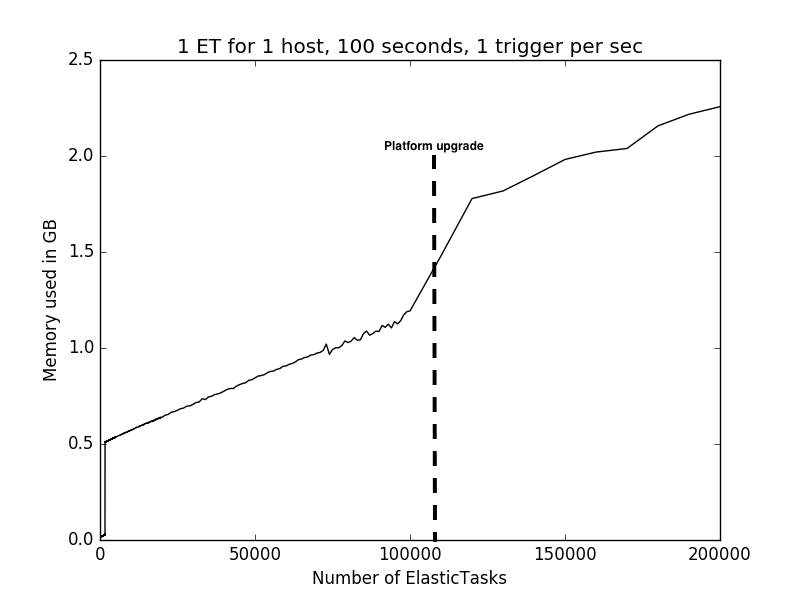
\includegraphics[width=\textwidth]{../plots/raw_perf_mem}
    		\caption{Raw performances Max Memory.}
    		\label{mem_raw}
    	\end{subfigure}%
    	\caption{Raw performances.}
    \end{figure}
    
    \figurename~\ref{time_raw} shows the CPU time (user + system time) while
    \figurename~\ref{mem_raw} shows the maximum memory used. To get the $x$ axis
    with the total number of microtasks you just have to multiply by 100. The
    platform was upgraded two times, at 1,600 from 2,000 hosts to 100,000, and
    then at 100,000 from 100,000 to 200,000. We can see that the deployment of
    the platform has nearly no impact on the time but account for about a half
    of the memory used if there is as much ETs as hosts. Apart from that, time
    and memory grows linearly depending of the ETs amounts and operations done.
    
    \paragraph{Experiment 2}
    \begin{figure}
    	\centering
    	\hspace*{-4em}
    	\begin{subfigure}[t]{0.6\textwidth}
    		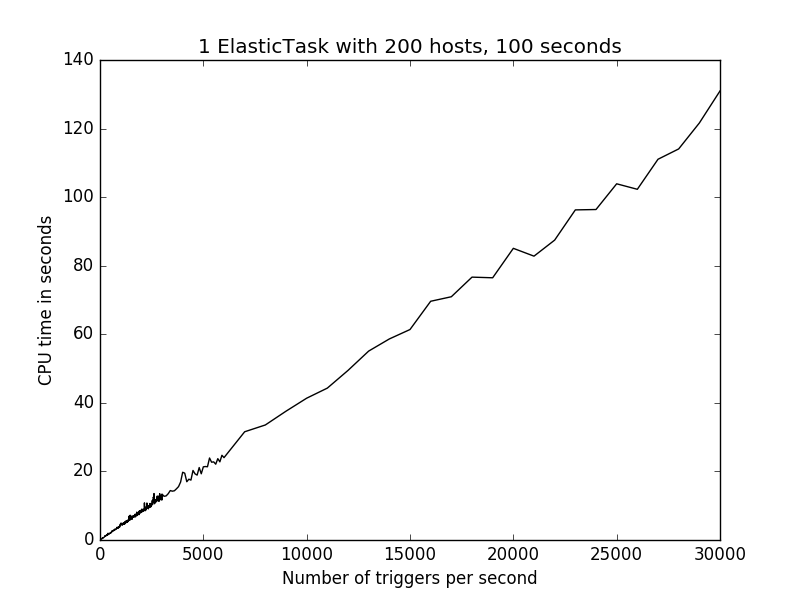
\includegraphics[width=\textwidth]{../plots/raw_perf_oneet_time}
    		\caption{Raw performances CPU time.}
    		\label{time_oneet_raw}
    	\end{subfigure}%
    	~
    	\begin{subfigure}[t]{0.6\textwidth}
    		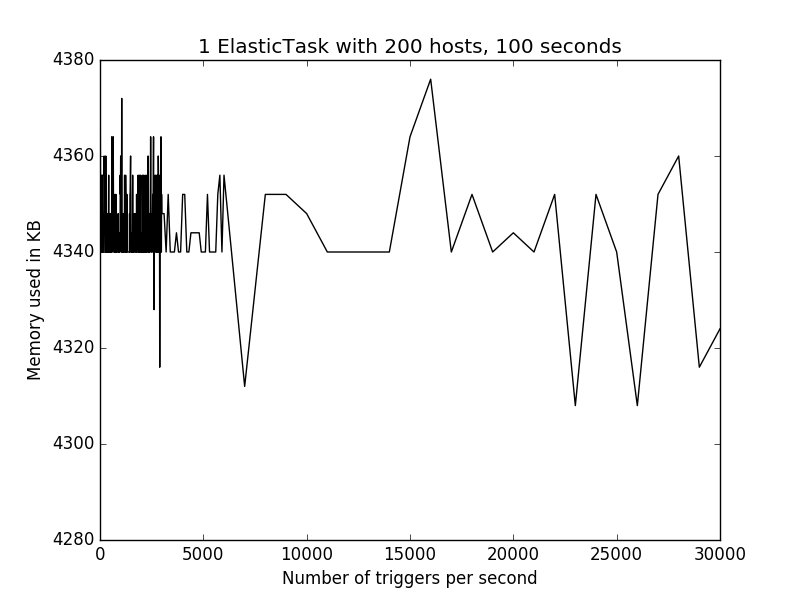
\includegraphics[width=\textwidth]{../plots/raw_perf_oneet_mem}
    		\caption{Raw performances Max Memory.}
    		\label{mem_oneet_raw}
    	\end{subfigure}%
    	\caption{Raw performances.}
    \end{figure}
        
    \figurename~\ref{time_oneet_raw} shows the CPU time and
    \figurename~\ref{mem_oneet_raw} shows the maximum memory used. To get the
    $x$ axis with the total number of microtasks you just have to multiply by
    100. As we don't touch the platform or application structure (we just touch
    its usage) the memory remains constant. As seen before the time is linear 
    with the number of microtasks and with about the same growing speed.
    
    What will create workload are the elastic tasks and the two way of 
    increasing the workload (increasing the number of microtasks) are to add 
    more elastic tasks or increase the ratio of triggering. For both this cases 
    time is linear on the total number of microtasks and memory will increase 
    depending on the size of the platform and app architecture while always 
    being moderate for an present-day computer. We did not focused on the 
    amount of flops a microtask has because in the end the simulator is just 
    doing a subtraction. Though you have to be careful to always have enough 
    resources because then microtasks are delayed and start to stack up. At 
    some point the simulator will have a hard and in the end it might crash 
    your computer because of an excessive usage of memory.
    
    %TODO say that we need a callback when there are too much and QoS isn't met
    
       
  \subsection{Real traces} \label{real_traces}
		Evaluating the use of traces feature has two goals. Show that it works and 
		similarly to \ref{raw_perf} we want to show that evaluations done in papers 
		are possible in a simulation.
  
    For that we used real traces from WorldCup 98 data access logs \cite{wc98}
    with a platform of 2,000 host and enough flops. \figurename~\ref{tab_traces}
    shows the results of a few executions. Again time and memory usage are
    reasonable for days of real time simulated (even though these traces are
    getting old and might not be as big as nowadays requests logs). Adding more
    hosts changed nothing except for the deployment of the platform as we have
    seen in \ref{raw_perf}.

		\begin{figure}
			\centering
	    \begin{center}
	     	\begin{tabular}{| l | c | c |}
	     		\hline
	     		Trace (\# of requests) & Time & Max Memory\\ 
	     		\hline
	     		test (1,000) & 0.14s & 13,484 KB\\
		      \hline
		      day 10 (1,522,111) & 50.82s & 13,876 KB\\
		      \hline
		      day 20 (6,326,015) & 229.62 & 14,472 KB\\
	     		\hline
	     	\end{tabular}
	    \end{center}
	    \caption{Execution of WorlCup 98 website traces.}
	    \label{tab_traces}
	  \end{figure}
  
  \subsection{Functionalities}
	  As we have determined the needs for cloud elasticity works experiments, we 
	  have to evaluate which ones are filled. Apart from performances which are 
	  addressed in \ref{raw_perf} and \ref{real_traces} there are left elastic 
	  actions, workload generation features, and system feedback. For various 
	  papers, \figurename~\ref{table_func} shows which needs are filled and which 
	  are not.
  
	  \begin{figure}
	  	\centering
	  	\begin{center}
	  		\begin{tabular}{| l | c | c |}
	  			\hline
	  			& Implemented & \cite{vasic2012dejavu}\\ 
	  			\hline
	  			Horizontal scaling & YES & \checkmark\\
	  			\hline
	  			Vertical scaling & YES & \checkmark\\
	  			\hline
	  			Workflow & YES & \\
	  			\hline
	  			Threshold & NO & \\  %TODO define threshold
	  			\hline
	  			Traces & YES & \\
	  			\hline
	  			Constant rates & YES & \\
	  			\hline
	  			Generating law & NO & $\times$ \\
	  			\hline
	  		\end{tabular}
	  	\end{center}
	  	\caption{Functionnal requirements of several scientific studies.}
	  	\label{table_func}
	  \end{figure}
  
	  For horizontal and vertical scalings, they can be performed by modifying the
	  list of hosts of an ET. To scale up you just have to add hosts and to scale
	  out you have to replace this list with different hosts. Concerning workflows
	  of tasks you can set the output function with a function that has access to
	  ETs you want to trigger and just trigger them in the function, with possibly
	  a multiplicative effect of the workload.
   

% \section{Future work} \label{futurework}
% generator law, add natively other kinds of workload instead of letting the 
% user do some kinds of hacks


\section{Related work} \label{sota}
According to the classification of the survey, a simulator should allow the
manipulation of scopes, the evaluation of the different purposes, make
possible the elastic actions and allow multiple providers.

At the moment no simulator article talks about dynamic workload. On the other
hand in the code of DCsim \cite{tighe2013towards} there was an interactive
task and in the code of CloudSim \cite{calheiros2011cloudsim} there was an
host with dynamic workload. There are some tools to generate artificial
workload like \cite{bodik2010characterizing} and they generally follow the
following steps. They have a thread that acts like clients/users and it makes
request over time and simulate thinking times of the users.

%On a less technical note, workloads are generally seen as a number of 
%requests per a certain interval of time.

Five papers in the survey used simulations. They used discrete event 
simulators (home-made or OMNeT++), used benchmarks like SPECjEnterprise2010 
to have close-to-reality hosts, and run real traces.
  

\section{Conclusion} \label{conclu}
During this internship we've studied which actions were taken by elastic clouds 
mechanisms. Then we searched what was done in simulations used for evaluations 
and other evaluations to come with a contribution that meets the needs of 
researchers. To prove that the contribution was good enough we evaluated it on 
some criteria.

For future works we would need a callback for the user to set a certain 
response time (a threshold) and allow him to react accordingly if this QoS level
is not met. For that we would just need to either set an alarm and turn it off
once the workload has been executed and if it is not then it stops it and
execute a user's function. That would be an online solution and an offline one
would be to just see how much time the workload took to be executed and let the
user react accordingly. Another feature that would be really useful is a
generating law. For an elastic task the date for the next triggering would be
based on a statistical function. That would get us even closer to simple and
simplistic setup for experiments. Finally, the microtasks we have used are
computing tasks. Users can set the flops amount to 0 and add more specific tasks
in an output function but this is too hack-y. Right now in SimGrid there is only
computing and network tasks and you can also simulate disk usage by seeing it as
a computing resource.

On a more personal note, this internship has allowed me to discover what a 
simulator was, what a research code looked like along with its development, the 
life in a research environment, and many more.


\section*{Acknowledgment}
Thanks to Martin Quinson and Anne-C\'ecile Orgerie for guiding and advising me 
during this internship. Also many thanks to Inria for hosting me.


\bibliographystyle{IEEEtran}
\bibliography{bibi}
\end{document}
